\chapter{معماری نمونه مطالعاتی برنامه اشتراک سفر}

\section{زمینه برنامه اشتراک سفر}
هدف ایجاد یک بازار برخط میان رانندگان و مسافران است تا از یک سمت نیاز مسافران برای یافتن رانندگانی که مقاصد و شرایط نزدیک به دلخواه آن برای سفر دارند رفع شود و از سوی دیگر رانندگان قادر باشند تا مسافران باب میل خود را از میان مسافرین انتخاب کنند.در این میان برنامه باید اطلاعات سفر ها را لحظه به لحظه رصد کند تا از بروز هر گونه مشکل جلوگیری شود.

معماری پیشنهادی برای چنین زمینه\LTRfootnote{Context} ای معماری \lr{micro-service} 
\cite{micro_a}
است تا با شکستن برنامه بر اساس عملکرد‌ها\LTRfootnote{Functionalities} به میکرو سرویس های متناظر، نیازهای کیفی و غیرکیفی را مرتفع سازد.به این صورت با شکستن برنامه به مولفه‌های تقریبا مستقل بر حسب منطق تجاری به برنامه قابلیت حمل، انعطاف‌پذیری، رشد و گسترش‌پذیری بیشتری داده می‌شود. نمونه معماری مورد نظر برای برنامه اشتراک‌گذاری خودرو را در شکل \ref{fig:trip} نمایش داده شده است \cite{micro_carpooling} .
در مورد بحث دردسترس‌پذیری در معماری میکروسرویس، تاب‌‌آوری\LTRfootnote{Resilience} مهم‌ترین فاکتور است؛ حفظ دسترس‌پذیری با مدیریت و مانیتورینگ صحیح سرویس‌ها امکان‌پذیر خواهد بود.گسترش‌پذیری در معماری میکروسرویس در گرو تخصیص بهینه منابع به سرویس ها توسط مولفه توزیع‌بار\LTRfootnote{LoadBalancer} است.

\section{معماری پیشنهادی}

الگو معماری میکرو‌سرویس‌ها روشی برای توسعه برنامه در قالب سرویس‌های کوچک است که هر کدام به صورت تقریبا مستقل فعالیت می‌کنند.این الگو امکان تحویل/استقرار مداوم\LTRfootnote{Continouse Delivery/Development} برنامه های پیچیده و بزرگ را فراهم می کند و همچنین به یک سازمان امکان می دهد تا به تدریج پشته فناوری خود را توسعه دهد.

\begin{figure}[htb]
\centering
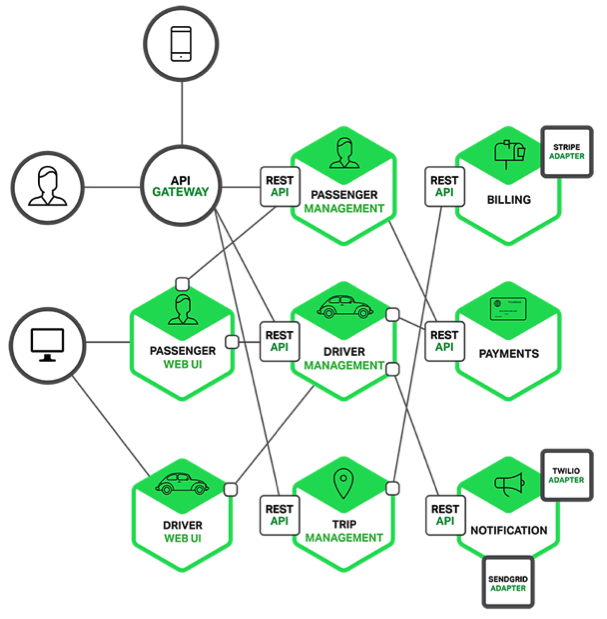
\includegraphics[scale=0.7]{trip.png}
\caption{ معماری میکروسرویس برنامه اشتراک سفر، عکس از \cite{micro_carpooling}}
\label{fig:trip}
\end{figure}

طبق معماری تعیین‌شده برنامه‌های سمت کاربر از طریق \lr{API Gateway} درخواست‌های خود را ارسال می‌کنند و سرویس‌ها در ارتباط با یکدیگر به درخواست‌های کاربران پاسخ می‌دهند.


\section{نیازمندی‌های پوشش‌داده شده توسط معماری}
در ادامه به تجزیه و تحلیل مشخصات معماری رایج برای الگوی معماری میکرو‌سرویس ها و میزان توانایی این الگو در رفع نیاز‌های کیفی پرداخته می‌شود.

چابکی و توانایی پاسخ سریع به تغییرات محیطی در کسب‌و‌کار‌های رقابتی نظیر صنعت حمل‌و‌نقل اهمیت بالایی دارد.با توجه به مفهوم واحدهای مستقل و کوچک در الگوی میکرو‌سرویس برنامه با چنین الگویی می‌تواند با کمترین هزینه تغییرات لازم را در خود اعمال کند و از قابلیت تغییر‌پذیری\LTRfootnote{Modifiability} بالایی برخوردار است.

به دلیل تفکیک عملکرد و دغدغه‌های تجاری در برنامه‌ها با الگوی میکرو‌سرویس، می توان تست را محدود کرد، و این امر باعث می شود که آزمایشات هدفمندتر انجام شوند. همچنین آزمون برای یک سرویس خاص بسیار آسان تر و عملی تر از نوشتن آزمون برای یک معماری \lr{Monolithic} است و چون در معماری میکروسرویس مولفه‌ها \lr{loosely coupled} هستند امکان این‌که یک تغییر در یک سرویس منجر به شکست سایر سرویس‌ها شود،کم است.

به دلیل ذات توزیع‌شده و نیاز به پیام‌رسانی تحت شبکه در الگوی میکروسرویس نوشتن سرویس‌ها با کارایی بالا در خروجی مناسب بسیار اهمیت دارد و یکی از چالش‌های استفاده از الگوی میکروسرویس حفظ کارایی در هنگام گسترش برنامه است اما در مقابل چالش کارایی گسترش‌پذیری برنامه تحت این الگو به راحتی صورت می‌پذیرد و با ساختار خود پیچیدگی مسائل رو با شکستن به ریز‌سرویس ها کاهش می‌دهد. همچنین وجود امکان ارتباط راحت با سرویس‌های دیگر نیز به قابلیت همکاری در این معماری نیز کمک می‌کند.

پویایی معماری میکرو سرویس این امکان را می‌دهد که بتوان به چالش‌های امنیت نیز پاسخ داد، با استفاده از این معماری می‌توان تمامی ارتباطات را رمز کرد، تمامی درخواست‌ها را احراز هویت کرد و به چالش‌های رمزگذاری و دنبال کردن نشست کاربران و جلوگیری از حملات منع سرویس با استفاده از فیلترها نیز پاسخ داد \cite{micro_secure} .

از انجا که در این معماری می‌توان رنج وسیعی از \lr{API} ها را برنامه ریزی کرد بنابراین در صورت طراحی مناسب \lr{API} ها می‌توان به نیازمندی‌هایی که موجب افزایش قابلیت استفاده کاربر می‌شود نیز پاسخ داد.

در پترن میکروسرویس هر سرویس  پایگاه داده  خود را دارد. با این وجود برخی از تراکنش‌های تجاری شامل سرویس های مختلفی هستند بنابراین به مکانیزمی برای اجرای تراکنش‌ها نیاز است. اجرای هر تراکنش تجاری که شامل چندین سرویس باشد یک \lr{Saga} است، در واقع \lr{Saga} شامل چندین تراکنش محلی است. هر تراکنش محلی که پایگاه داده یک سرویس را به روز می کند،یک پیام یا رویدادی را منتشر می کند تا تراکنش محلی بعدی را در \lr{saga} آغاز کند.یکی از خوبی های استفاده از \lr{Saga} این است که اگر یکی از تراکنش‌های محلی شکست بخورن \lr{saga} مجموعه اقداماتی را جهت \lr{rollback} تراکنش‌ها انجام می‌دهد.\cite{saga}
\section{نتیجه‌گیری}
معماری میکرو‌سرویس پیشنهادی، مزایای زیر را با خود به همراه خواهد داشت:
\begin{itemize}
\item
اول ، این که میکرو‌سرویس مشکل پیچیدگی زیاد را حل می کند. پترن میکروسرویس به عنوان مثال یک معماری یکپارچه\LTRfootnote{Monolithic} را به مجموعه ای از خدمات تجزیه می کند و بنابرین با حفظ  کل عملکرد سیستم، برنامه به چند بخش سرویس قابل مدیریت تقسیم شده است و هر سرویس دارای یک مرزبندی کاملاً  مشخص به واسطه‌ی \lr{RPC} یا \lr{message-driven API} است. الگوی معماری میکروسرویس‌ها سطحی از ماژولاریتی\LTRfootnote{Modularity}را اعمال می کند که دستیابی به آن با پترین یکپارچه بسیار دشوار است. در نتیجه ، توسعه سرویس‌ها بسیار سریعتر و درک و نگهداری آنها بسیار آسان تر است. 
\item
دوم ، این معماری امکان توسعه هر سرویس را به طور مستقل، فراهم می‌کند و تیم‌های توسعه حول سرویس‌ها شکل می‌گیرند. توسعه دهندگان،  به شرطی که این‌که قرارداد ها پیرامون \lr{API} ها را رعایت کنند، در انتخاب هرگونه فناوری آزاد هستند؛ البته ، اکثر سازمان ها مایلند از هرج و مرج کامل جلوگیری کرده و گزینه های فناوری را محدود سازند. با این حال ، این آزادی به معنای آن است که توسعه دهندگان دیگر ملزم به استفاده از فن آوری های احتمالاً منسوخ شده ای که در آغاز یک پروژه جدید وجود داشته است نیستند و هنگام نوشتن سرویس جدید ، امکان استفاده از فناوری‌‌های روز را دارند. علاوه بر این ، از آنجا که خدمات نسبتاً کوچک هستند، بازنویسی یک سرویس قدیمی با استفاده از فناوری روز امکان پذیر است. 
\item
سوم ، در الگوی معماری میکروسرویس می‌توان هر میکرو‌سرویس را مستقلاً مستقر\LTRfootnote{Deploy}کرد. توسعه دهندگان هرگز نیازی به هماهنگی در استفاده از تغییراتی ندارند که از منظر سرویس محلی باشد.
\item
چهارم ، الگوی معماری میکروسرویس ها مقیاس بندی هر سرویس را به طور مستقل امکان پذیر می کند. 
\item
پنچم، سرویس‌ها به دلیل اندازه کوچک و وظیفه مشخص بسیار آزمون پذیر هستند. 
\end{itemize}
در کنار مزایایی که یک معماری با خود به همراه دارد نقاط ضعفی نیز وجود خواهند داشت که باید در ادامه بر اساس \lr{ASR} های مطرح برای ذی نفعان با استفاده از سایر پترن‌ها و تاکتیک‌ها در معماری به حل آن‌ها پرداخته شود.از جمله معایب استفاده از معماری میکروسرویس می‌توان به موارد زیر اشاره کرد:
\begin{itemize}
\item
اول، تاکید زیاد بر اندازه‌ی سرویس ها و مشخص نبودن دقیق اندازه مناسب سرویس ها از جمله معایبی است که در ابتدای کار با میکروسرویس‌ها با آن برخورد خواهید داشت.
\item
دوم، در این پترن،تعيين حدود و مرزبندی میانن سرويس ها مشكل است. 
\item
سوم، به دلیل ماهیت توزیع شده پیچیدگی‌های جدیدی به سیستم اضافه می‌شود.
\item
چهارم، كارايي پائين ( ارتباطات شبكه اي) در معماری میکروسرویس مشهود است.
\end{itemize}

استفاده از معماری میکروسرویس به تیم‌ها اجازه می‌دهد تا با سرعت افزایش حجم بازار هدف خود را منطبق سازند و از طرفی پا به پای پیشرفت‌های تکنولوژی حرکت کرده و خود را به روز کنند.